% Yeban User Guide — Chapter 9: Shortcuts and Command Reference (English)
% T-DOC-001 chapter-by-chapter delivery, written ahead of the CH09 task.
% Sources: cli.rs SHORTCUTS (the single authoritative table), help.rs in-app reference,
% docs/manual/README.md writing rule (no second hand-copied key table).

\chapter{Shortcuts and Command Reference}
\label{ch:shortcuts}

\begin{quote}
以无厚入有间，恢恢乎其于游刃必有余地矣。
\end{quote}

Source: Zhuangzi, “The Secret of Caring for Life” (《庄子·养生主》). Translation: “Where there is no thickness to enter what has gaps, there is ample room for the blade to move.”

Shortcuts make frequent actions effortless; once the hands know the way, the mind can stay with the music.

Yeban has a single authoritative shortcut policy table: the one shown under Help $\to$
Shortcuts, which is the same table printed by \texttt{yeban-app --print-shortcuts}.
This chapter groups common keys by workflow as a memory aid; it is not a second
authoritative table — for the full list and implementation status, use the in-app
reference.

\section{The Policy Table Shared with In-app Help}

\subsection{Why this chapter does not copy the full table}

The policy table evolves: it marks row by row which keys are implemented and which are
"bound but not yet implemented" in the host. A hand-copied table goes stale quickly and
can turn "not implemented" into "available". So this chapter does only two things:
explain the canonical key notation, and pick out high-frequency operations by workflow.

\subsection{Canonical notation and platform folding}

The table keeps the cross-platform canonical form \texttt{Cmd/Ctrl+}: on macOS it
renders as \texttt{Cmd+}, elsewhere as \texttt{Ctrl+}. So \texttt{Ctrl+S} on Windows
and \texttt{Cmd+S} on macOS are the same canonical binding. A key marked "(not
implemented)" is bound and resolves to an action, but the host has no implementation
yet and rejects the press — the key is not broken.

\section{Common Keys by Workflow}

The keys below all come from the policy table, grouped in the order you tend to work.

\subsection{Projects and editing}

\begin{description}
  \item[Cmd/Ctrl+N] New MIDI synth track.
  \item[Cmd/Ctrl+O] Open project.
  \item[Cmd/Ctrl+S] Save project; Cmd/Ctrl+Shift+S save as.
  \item[Cmd/Ctrl+Z] Undo; Cmd/Ctrl+Shift+Z redo.
  \item[Tab] View switch (canvas focus only); F5 Session view, F6 Arrangement view.
\end{description}

\subsection{Arranging and editing clips}

\begin{description}
  \item[Space] Play/pause; Shift+Space resume from cursor.
  \item[Enter] Return to start; C cycle playback toggle.
  \item[Cmd/Ctrl+T] Split selected clip at the playhead.
  \item[Cmd/Ctrl+C / V / X] Copy / paste / cut clips.
  \item[Cmd/Ctrl+= / -] Zoom the timeline horizontally in/out.
  \item[Cmd/Ctrl+Up/Down] Zoom tracks vertically out/in.
\end{description}

\subsection{Bottom console and panels}

\begin{description}
  \item[P / F7] Piano roll; X / F8 mixer console; F9 device rack; F3 console device stack.
  \item[I] Toggle the left inspector.
  \item[Cmd/Ctrl+Shift+A] Show automation lanes.
  \item[Cmd/Ctrl+Shift+B] Open the unified browser (sounds/samples/presets/effects).
  \item[E] Toggle editor view.
\end{description}

\subsection{Recording and other}

\begin{description}
  \item[R] Recording on/off.
  \item[Cmd/Ctrl+Shift+H] Time Machine.
  \item[Esc] Close the command palette / hotspot overlay.
\end{description}

\subsection{The IME exception}

In text input and IME composition mode, every key except F5/F6 is swallowed by the
input method and does not trigger the actions above — deliberately, so typing does not
fire shortcuts. The policy table has separate columns explaining "canvas focus"
versus "text input + IME composition".

\screenshot{ch09-shortcuts-panel}{The Help $\to$ Shortcuts panel showing canonical form, keys, actions and implementation status columns}

\begin{figure}[htbp]
\centering
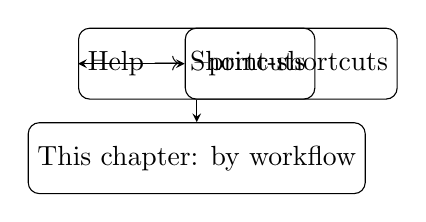
\begin{tikzpicture}[node distance=1.2cm, >=stealth,
    box/.style={draw, rounded corners, align=center, minimum width=2.2cm, minimum height=0.9cm}]
  \node[box] (a) {Help $\to$ Shortcuts};
  \node[box, right of=a] (b) {--print-shortcuts};
  \node[box, below of=a] (c) {This chapter: by workflow};
  \draw[<->] (a)--(b); \draw[->] (a)--(c);
\end{tikzpicture}
\caption{The authoritative source is the one policy table behind the in-app reference and \texttt{--print-shortcuts}; this chapter is only a guide}
\label{fig:ch09-shortcut-source}
\end{figure}

\section{Help Topic Mapping}

\begin{table}[htbp]
\centering
\caption{Sections of this chapter $\to$ in-app help anchors}
\label{tab:ch09-help}
\begin{tabular}{ll}
\hline
Section & Help topic \\
\hline
Shared policy table / notation & \texttt{shortcuts-policy-table} \\
Projects and editing & \texttt{shortcuts-project-edit} \\
Arranging and clips & \texttt{shortcuts-arrange} \\
Console and panels & \texttt{shortcuts-panels} \\
Recording and other & \texttt{shortcuts-record-misc} \\
IME exception & \texttt{shortcuts-ime-exception} \\
\hline
\end{tabular}
\end{table}

\paragraph{What you will be able to do} Find high-frequency keys by workflow, understand the \texttt{Cmd/Ctrl+} platform folding, and know that the full list lives in the in-app reference, not this chapter.

\paragraph{Hands-on exercise} Open Help $\to$ Shortcuts and pick three keys from this chapter that you use often but know less well; run \texttt{yeban-app --print-shortcuts} and confirm it shows the same bindings; finally, using only the keyboard, do "open project $\to$ split a clip $\to$ save".
